\newpage
\section{Projektplanung}

\subsection{Risikobewertung}

Alle bekannten Risiken von dem Projekt sind in folgenden Tabelle aufgelistet.
Dabei hat jedes Risiko folgende Attribute:
\begin{itemize}
    \item \textbf{Titel + Beschreibung}: Beschreibung des Risikos
    \item \textbf{Verantwortlich} Welche Gruppe dafür Verwantwortlich ist (INF=Informatik, MT=Mechaniker, ET=Elektroniker).
    \item \textbf{Kategorie}: In welcher Kategorie sich das Risiko befindet.
    \item \textbf{Ursachen}: Was passieren muss, damit das Risiko eintreffen kann.
    \item \textbf{Bewertung des Risikos}: Eintrittswahrscheinlichkeit, Auswirkung und Risiko Bewertung ohne Massnahmen
    \item \textbf{Massnahmen zur Risikominimierung}: Massnahmen um die Eintrittswahrscheinlichkeit oder Auswirkung zu minimieren.
    \item \textbf{Korrekturmassnahmen}: Was gemacht werden soll, wenn das Risiko trotzdem Eintrifft
    \item \textbf{Erfolgsfaktoren}: Beschreibt das Verhalten bei erfolgreicher Risikomitigation
    \item \textbf{Erneute Bewertung des Risikos}: Eintrittswahrscheinlichkeit, Auswirkung und Risiko Bewertung mit den definierten Massnahmen
\end{itemize}
\begin{landscape}
\scriptsize
\begin{longtable}{|c|p{4cm}|p{7cm}|c|c|p{4cm}|c|c|c|}
\hline
ID & Title & Beschreibung & Ver. & Kategorie & Ursachen & EW & AW & Bew.  \\
\hline
R1 & Grip-Verlust normale Räder & Das Fahrzeug schleift über den Boden & MT & Mechanisch & Fahrzeug verliert Grip \\
\hline
R2 & Liniensensor falsche Daten & Der Liniensensor erkennt die Fugen als Führungslinie & ET+INF & Elektrisch & Fahrzeug folgt der Fuge \\
R3 & Motorenposition ungenau & Für Rückstellen des Hinderniss ungenau Positonswerte & ET & Elektrisch & Hinderniss nicht innerhalb 2 cm \\
\hline
R4 & Distanzmessung fehlerhafte Daten & Für die Erkennung der Distanz, des Hinderniss, könnten falsche Messwerte eine ungewollte Aktion ausführen & ET & Elektrisch & Fahrzeug führt Hindernissbewältigung aus ohne ein Hinderniss \\
\hline
R5 & Datenverlust & Verlust von Projektdaten/Forschungsergebnissen & INF & Projekt & Server offline \\
\hline
R6 & Lieferschwierigkeiten & Teile, die bestellt werden haben Lieferverzögerung, was zur Verzögerung im jeweiligen Test-/Integrationsprozess führt & Market & & Längere Lieferzeiten/Keine Lieferzeiten angegeben \\
\hline
R7 & Software-Absturz & Software crasht während Einsatz & INF & Software & Prozess wird unerwartet beendet \\
\hline
R8 & Verlust Sensorkommunikation & Die Kommunikation zwischen Sensorik und Software ist gestört & ET+INF & Software & Fehlerhafte Daten oder fehlende Daten \\
\hline
R9 & Software zu anspruchsvoll für Computer & Die Leistung des Computers reicht nicht für die Echtzeitverarbeitung der Algorithmen & INF & Software & Software-Lags, langsame Reaktionszeit \\
\hline
R10 & Pylone wird überfahren & Eine Pylone wird nicht erkannt und überfahren & ET+INF & Elektrisch & Pylone wird nicht erkannt \\
\hline
R11 & Unscharfe Bilder während Fahrt erschweren Objekterkennung & Die Kamera bewegt sich während der Fahrt zu stark und liefert unscharfe Bilder & MT+INF & Software & Objekterkennung findet keine Objekte oder an falschen Orten \\
\hline
R12 & Fokus der Kamera umfasst nicht ganzen benötigten Bereich & Bilder enthalten unscharfe Teile, da die Focus Range nicht den ganzen benötigten Bereich umfasst. (Von Fahrzeug zu nächstem Punkt (Max 2m)) & ET+INF & Elektrisch & Teile des Bilds unscharf und Objekte werden nicht korrekt erkannt \\
\hline
R13 & Grip Verlust Omni und Mecanum & & & Mechanisch & Fahrzeug verliert Grip bei den Fugen \\
\hline
R14 & Anzahl GPIO & Die Steuerungselektronik hat eine begrenzte Anzahl IN/OUT Pins & ET & Elektrisch & Sensorinformationen können nicht gelesen werden \\
\hline
R15 & Verschiebung bei Drehung & Mit dem Fahrantrieb kann keine genaue Drehung an Ort und Stelle realisiert werden, um das Fahrzeug mit dem aufgenommenen Hindernis zu wenden. & MT & Mechanisch & Fahrzeug schiebt zur Seite bei Drehung \\
\hline
\end{longtable}

\begin{longtable}{|c|c|c|c|p{6cm}|p{4cm}|p{4cm}|c|c|c|}
\hline
ID & Massnahmen Risikominderung & Korrekturmassnahmen & 
Erfolgsfaktoren & EWM & AWM & BewM.
\\ \hline
R1 & Possible & Moderate & 9 & Auf Mensaboden testen & Andere Räder/Geschwindigkeit anpassen & Fahrzeug hat Grip & Unlikely & Minor & 4 \\ \hline
R2 & Likely & Major & 16 & Kalibrierung des Sensors, Abgleich mit Kamera. Befahren einer Linie nur, wenn Punkt oder Hindernis am Ende erkannt & Not-Aus verwenden & Fahrzeug folgt Führungslinie & Unlikely & Critical & 10 \\ \hline
R3 & Possible & Moderate & 9 & Langsame Fahrt bei Positioierung & Hallsensor, Drehgeber, Schrittmotor, Beschleunigungssensor & Hinderniss innerhalb der 2 cm Toleranz & Unlikely & Minor & 4 \\ \hline
R4 & Unlikely & Minor & 4 & Distanzwert muss längere Zeit konstant bleiben & Zweiter Sensor zum Vergleich verbauen & Fahrzeug führt Hindernissbewältigung nur bei einem Hinderniss aus & Remote & Minor & 2 \\ \hline
R5 & Unlikely & Critical & 10 & Regelmässige Backups erstellen & Daten aus Backups wiederherstellen & Daten sind zugänglich und schnell wiederherstellbar & Unlikely & Minor & 4 \\ \hline
R6 & Possible & Major & 12 & Frühzeitig Bestellen, alternative Teile/Quellen suchen & bei alternativen Quellen bestellen, Alternative Teile nutzen & Teile können zeitnah verwendet verbaut werden & Possible & Moderate & 9 \\ \hline
R7 & Unlikely & Critical & 10 & Gutes Testen des Codes und Failsafe einbauen, der bei Absturz ausgeführt wird. Aktuellen Zustand zwischenspeichern & Not-Aus verwenden & Fahrzeug kann nach Absturz von alleine wieder starten und fortfahren, ohne, dass das Fahrzeug die Linien verlässt & Remote & Critical & 5 \\ \hline
R8 & Unlikely & Critical & 10 & Sicheres verbauen und Testen der Sensoren. Nominalwerte prüfen und Fehlerzustände definieren, um diese erkennen zu können. In solchen Fällen Neueinstellung/Kalibrierung durchführen & Wege in Software haben, um auch mit fehlender Sensorik die Aufgabe zu erfüllen. & Fahrzeug kann trotz fehlerhafter oder fehlender Sensorikdaten Aufgabe erfüllen & Unlikely & Moderate & 6 \\ \hline
R9 & Possible & Major & 12 & Software von Beginn auf für Plattform optimiert bauen. Keine Bewegung des Fahrzeugs, wenn Fahrsteuerung überlastet. & Akzeptieren und langsamer fortsetzen & Fahrzeug kann trotz langsamer Laufzeit die Aufgabe lösen & Possible & Moderate & 9 \\ \hline
R10 & Possible & Critical & 15 & Frühes Training und Testing für Pylonenerkennung mit Simulation oder real world data, Backup-Sensor, der bei Nichterkennen von nahem Hindernis Alarm schlägt & Not-Aus verwenden & Das Fahrzeug erkennt Pylonen und fährt sie nicht um & Remote & Critical & 5 \\ \hline
R11 & Likely & Major & 16 & Bildaufnahme nur bei stehendem Fahrzeug. Training mit verschwommenen Bilddaten. Dafür frühe Datenaufnahme nötig & Fahrzeug für längere Zeit stehen lassen, bis scharfe Bilder da sind & Das Fahrzeug erkennt Objekte und kann mit scharfen Bildern arbeiten & Unlikely & Major & 8 \\ \hline
R12 & Possible & Moderate & 9 & Im Vorfeld Fokus-Range prüfen und frühzeitig testen. Training mit verschwommenen Bilddaten & Software auf Fälle anpassen, bei denen Fokus-Bereich nicht reicht. & Fahrzeug kann Objekte richtig erkennen & Unlikely & Minor & 4 \\ \hline
R13 & Likely & Major & 16 & Testen der Räder & Mit Sensoren Position ausgleichen, dafür eine genaue Position des Fahrzeugs benötigt & Fahrzeug ist an der gewünschten Position & Possible & Moderate & 9 \\ \hline
R14 & Possible & Critical & 15 & & & & & & \\ \hline
R15 & Possible & Critical & 15 & Testen & Zusatzfunktion: abbocken und drehen des Fahrzeuges. & Fahrzeug dreht an fixer Position & & & \\ \hline
\end{longtable}

\normalsize
\end{landscape}


\addtocounter{subsection}{1}
\addcontentsline{toc}{subsection}{ TODO.1   Projektplan}
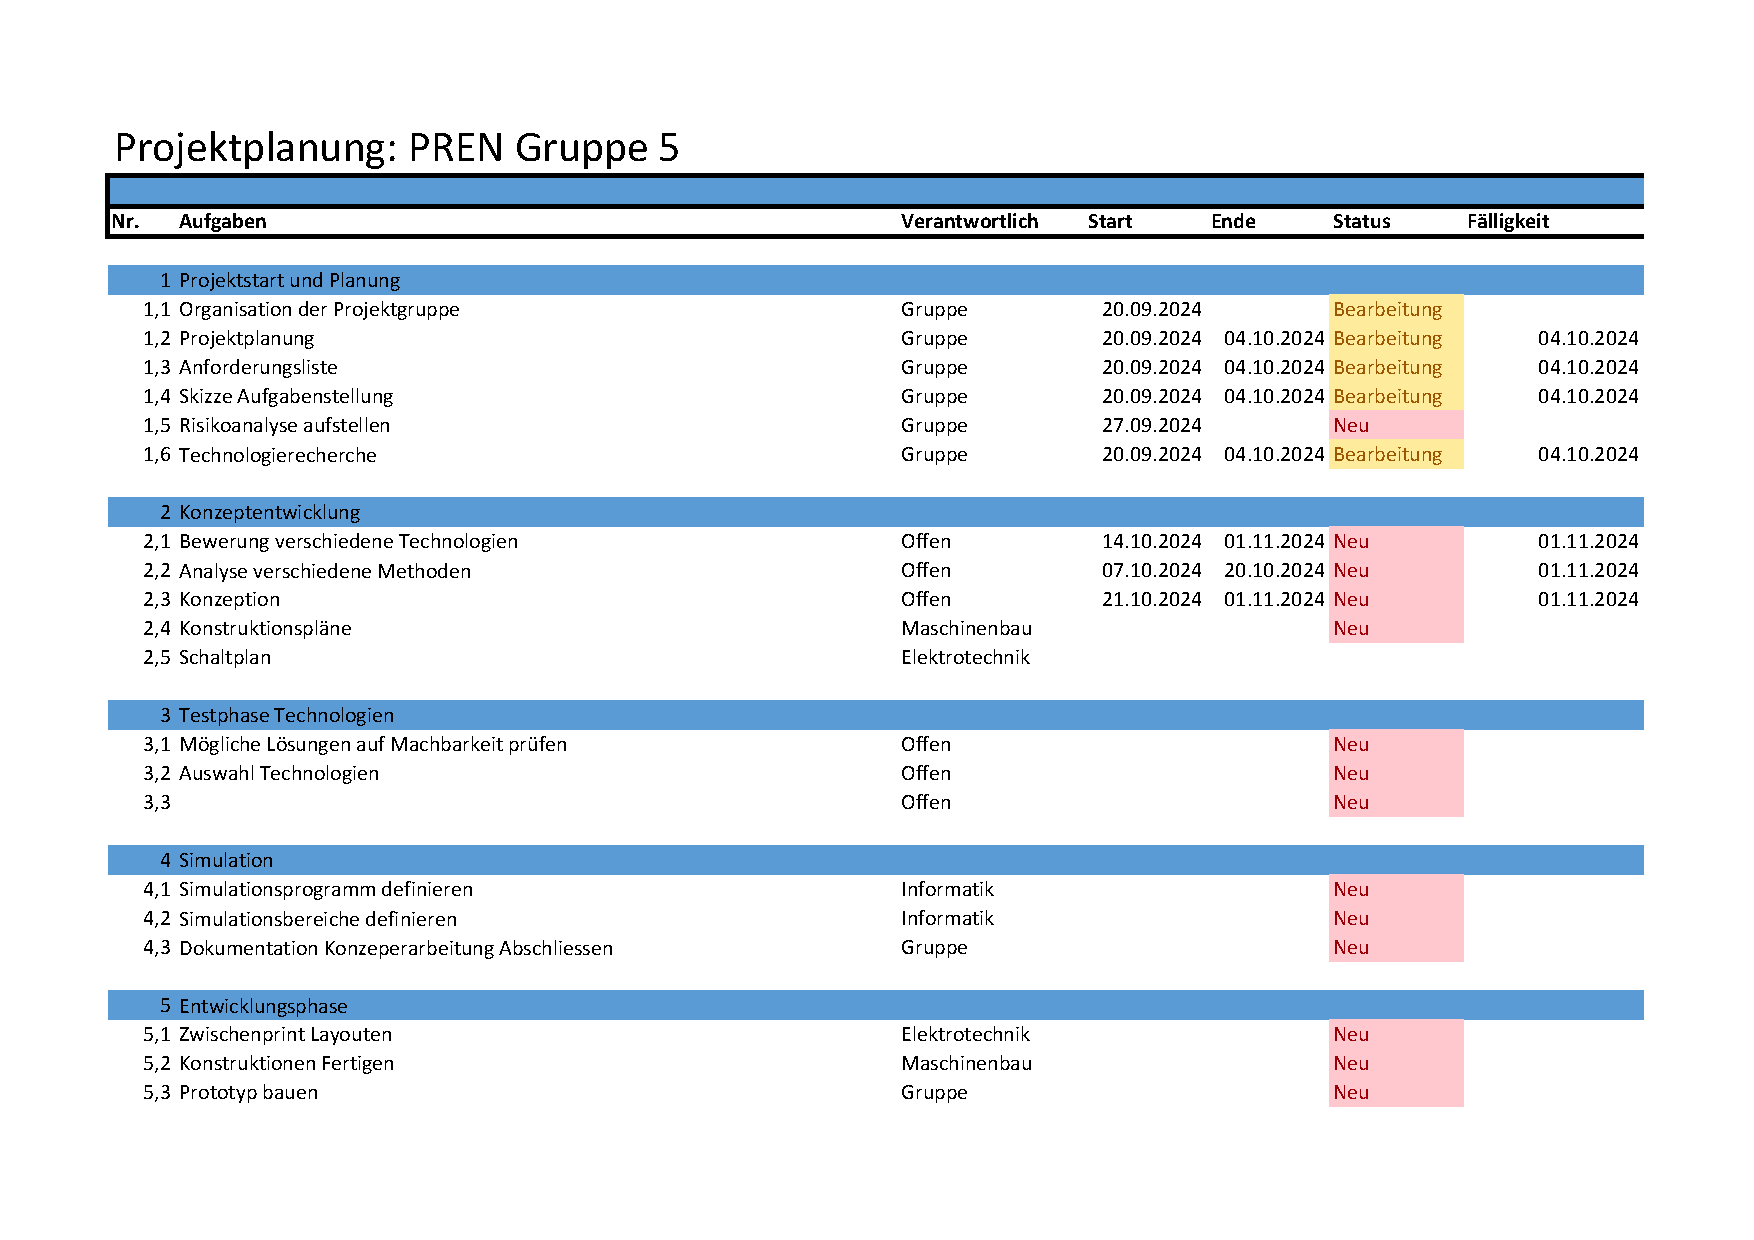
\includepdf[
  landscape=true,
  pages={1-},
  scale=0.9,
  pagecommand={\pagestyle{fancy}}
]{assets/Projektplan.pdf}

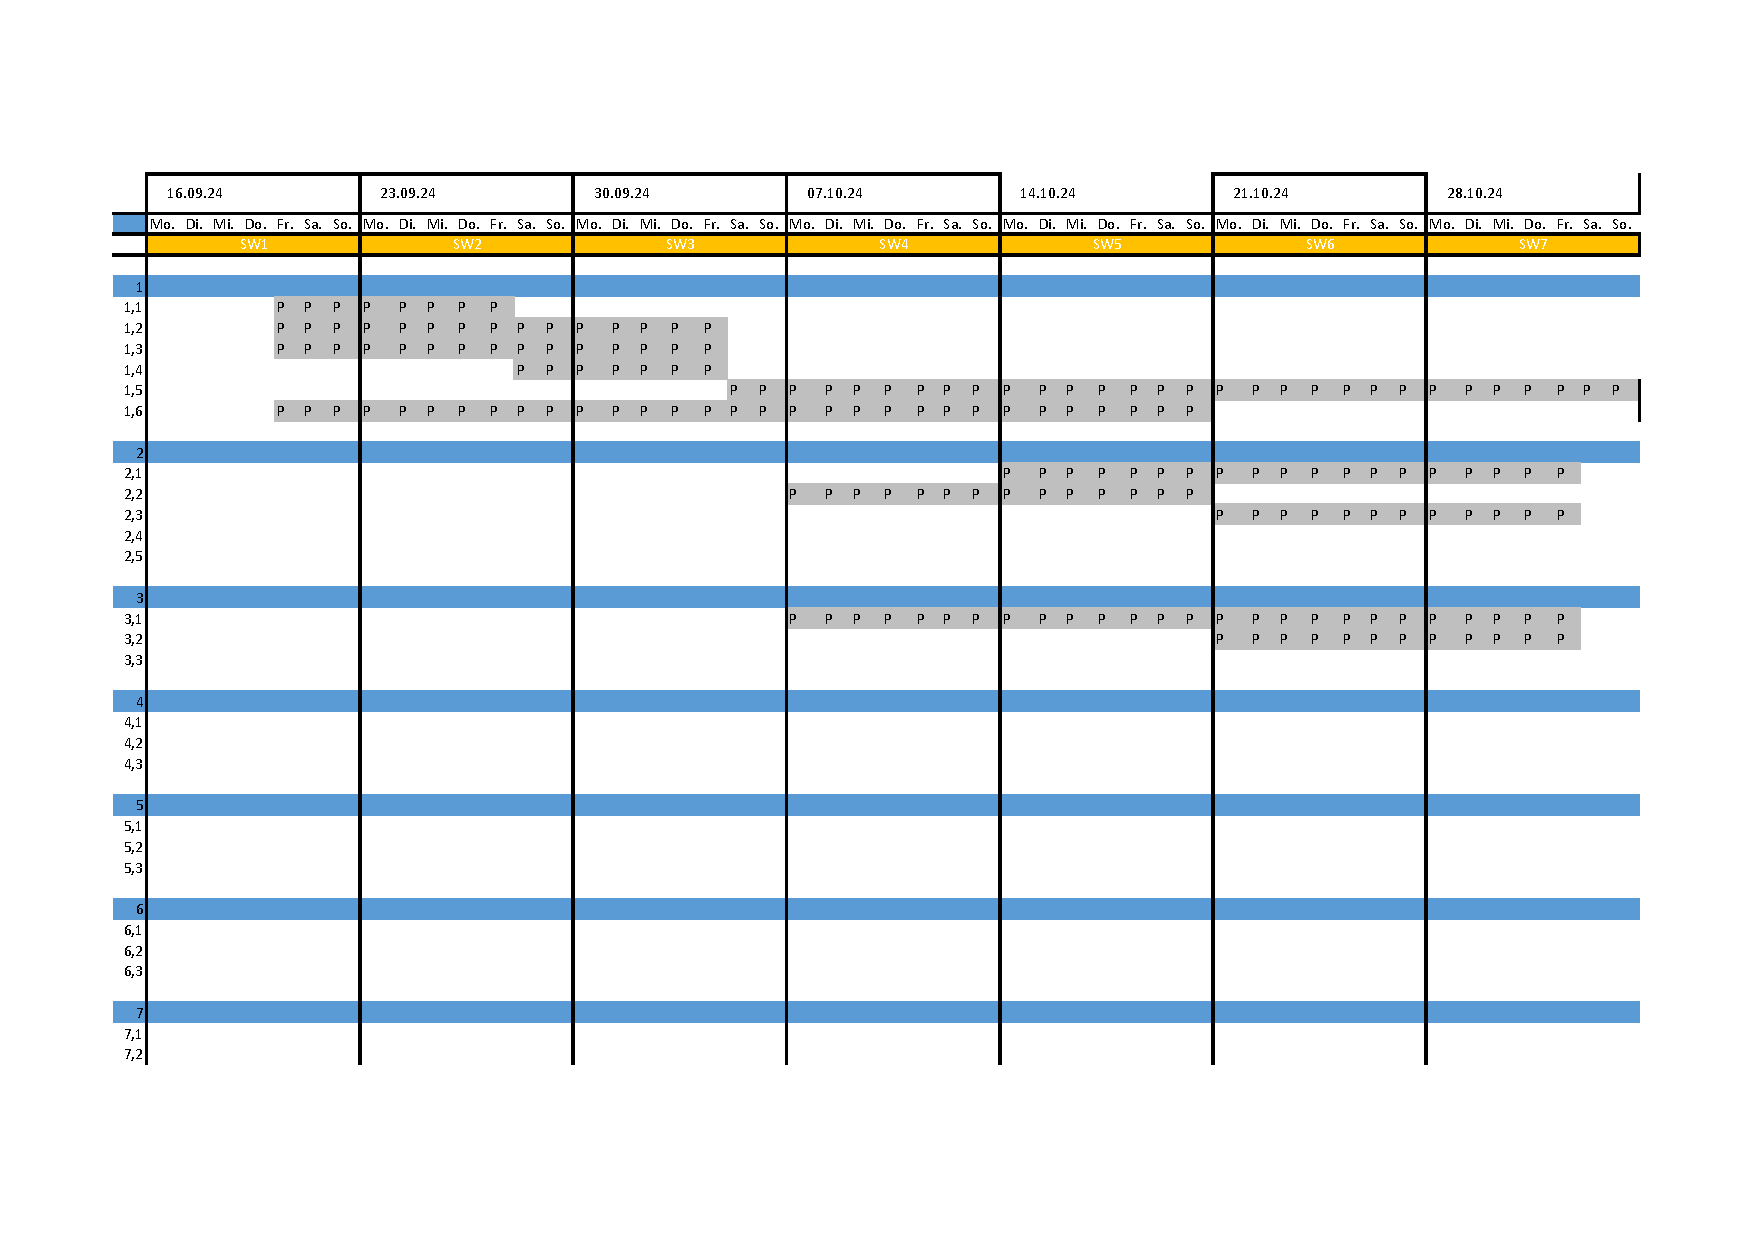
\includepdf[
  landscape=true,
  pages={1-},
  scale=0.9,
  pagecommand={\pagestyle{fancy}}
]{assets/Zeitplan.pdf}
